\chapter{Ermittlung der Architekturanforderungen}
Da die Software Architektur auf den Anforderungen basiert und viel wichtiger \glqq den gestalterischen Spielraum des Architekten\grqq \cite[S. 103]{softarch} begrenzt, kann davon abgeleitet werden, dass sowohl die Qualität der Architektur als auch die Akzeptanz des Systems wesentlich von den bereits im Vorfeld ermittelten Parametern abhängt. Das bedeutet wiederum, dass für die Klärung der Ausgangsfrage - Wie kommt man von Anforderungen auf eine gute Architektur - auch der Anforderungsprozess eine wichtige Rolle spielt.

Da der Anforderungsprozess ein an sich eigenes, sehr großes Themengebiet darstellt, wird hier jedoch nur auf die Ausgangsartefakte eingegangen, welche später im Architekturprozess referenziert werden. Zu diesen Parametern zählen nicht nur die Daten, AkteurInnen und Usecases, sondern auch die vorgegebenen nicht funktionalen Anforderungen.

Die Entwicklung der meisten Software Projekte ist oft ein dynamischer und agiler Prozess. Während des Entwicklungsprozesses werden oft Änderungen eingebracht und neue Anforderungen aufgestellt  \cite[S. 6-7, S. 37]{effektiv}. Auch führt die Komplexität des Systems und das Wissen des/der KundIn dazu, dass nach der Erhebung der initialen Anforderungen nicht alle Parameter vollständig bekannt sind. Dies wiederum führt mehr oder weniger dazu, dass der Anforderungsprozess während der Entwicklung der Architektur nicht als abgeschlossen gesehen werden kann und der/die KundIn verfügbar sein muss.

Aufgrund der Zehner-Regel der Fehler \cite[S. 154]{fehler} ist es zwar wichtig, möglichst viele Parameter schon so früh wie möglich zu kennen, jedoch führt dies in manchen Fällen zu einem verhältnismäßig zu hohem Aufwand. Zum Beispiel ist es wichtig und interessant die Schadenskosten zu kennen, welche nach einem unberechtigten Zugriff oder Manipulation von Daten durch die AkteurInnen auftreten können, jedoch erfordert dies eine komplette Gegenüberstellung von allen Daten und AkteurInnen in sämtlichen möglichen Szenarien: Bearbeiten, Erstellen, Löschen und Lesen. Ein Großteil dieser Kombinationen kann jedoch schon nach einer initialen, kurzen Phase der Aufspaltung in Netzwerke ausgeschlossen werden, weil bestimmte AkteurInnen keinen Zugriff mehr auf bestimmte Komponenten haben. Deswegen wird auf diese Szenarien erst nach einer kurzen, initialen Architekturphase eingegangen.

\section{Ermittlung der Usecases}
Die Usecases werden zusammen mit dem/der KundIn ermittelt. Daraus wird schlussendlich ein Usecasediagramm erstellt, welches alle AkteurInnen und Nachbarsysteme beinhaltet. Dies ist wichtig für das Kontextdiagramm, welches auch im Anforderungsprozess erstellt wird und die Ausgangsbasis für die Architektur darstellt.

\begin{figure}[!htbp]
    \centering
    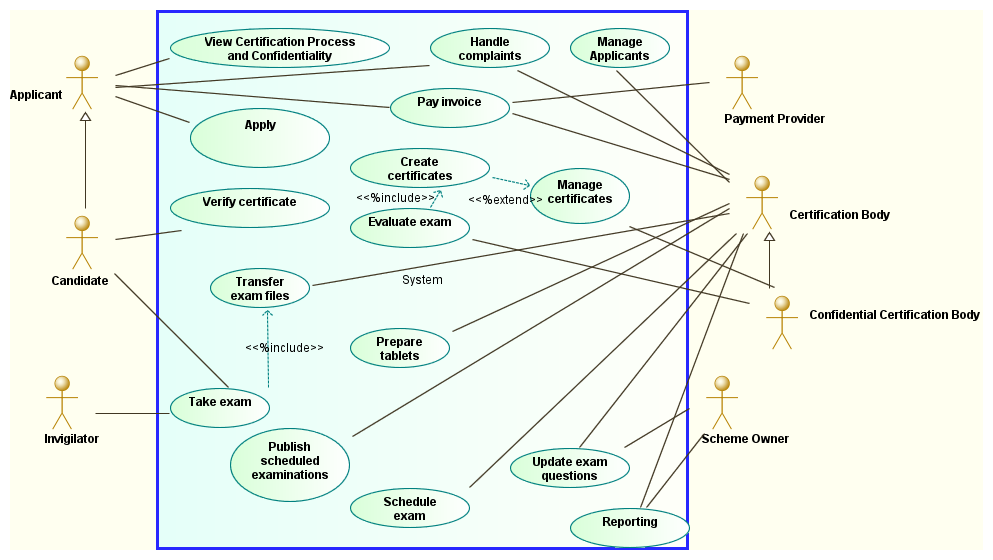
\includegraphics[scale=0.4]{uml/usecase.png}
    \caption{Aus den mit dem/der KundIn ermittelten Usecases wird ein Usecasediagramm erstellt}
\end{figure}

\subsection{Erweiterte Dokumentation der Usecases}
Parallel zur Erstellung des Usecasediagramms werden zusätzliche Parameter und Beschreibungen für jeden Usecase aufgenommen, welche im eigentlichen Diagramm nicht oder nur umständlich zu modellieren, aber wichtig für die Erstellung der Architektur sind.
Dafür wird ein Anforderungstemplate, auch Usecasebeschreibung genannt, verwendet \cite[S. 214]{reqman}, welches aufbauend auf einer Grundversion \cite[Abbildung 8.14, S. 215]{reqman} erweitert wird und für jeden Usecase folgende Angaben aufnimmt:

\begin{itemize}
  \item Id: eine eindeutige Bezeichnung, welche verwendet wird, um den Usecase zu referenzieren
  \item Actor: eine Auflistung aller TeilnehmerInnen des Usecases
  \item Description: eine kurze Beschreibung des Usecases
  \item Preconditions: eine Auflistung von Vorbedingungen für den Usecase
  \item Postconditions: eine Auflistung von Nachbedingungen für den Usecase
  \item Normal Course of Events: eine Beschreibung des Standardablaufes
  \item Alternative Courses: Auflistung von Erweiterungen oder zusätzlichen Pfaden des Usecases
  \item Exceptions: Beschreibung von diversen Ausnahme- und Fehlerfällen
  \item Assumptions: Annahmen, unter welcher der Usecase beschrieben wird
  \item Priority: eine Gewichtung, wie wichtig der Usecase ist: Low, Medium oder High
  \item Related Usecases: eine Auflistung von verwandten Usecases
  \item Notes: sonstige Anmerkungen
\end{itemize}

Sind die Abläufe komplexer, können Aktivitätsdiagramme verwendet werden, um Diese wie zB. in Abbildung \ref{fig:takexdet} verständlicher darzustellen \cite[S. 215]{reqman}:

\begin{figure}[H]
    \centering
    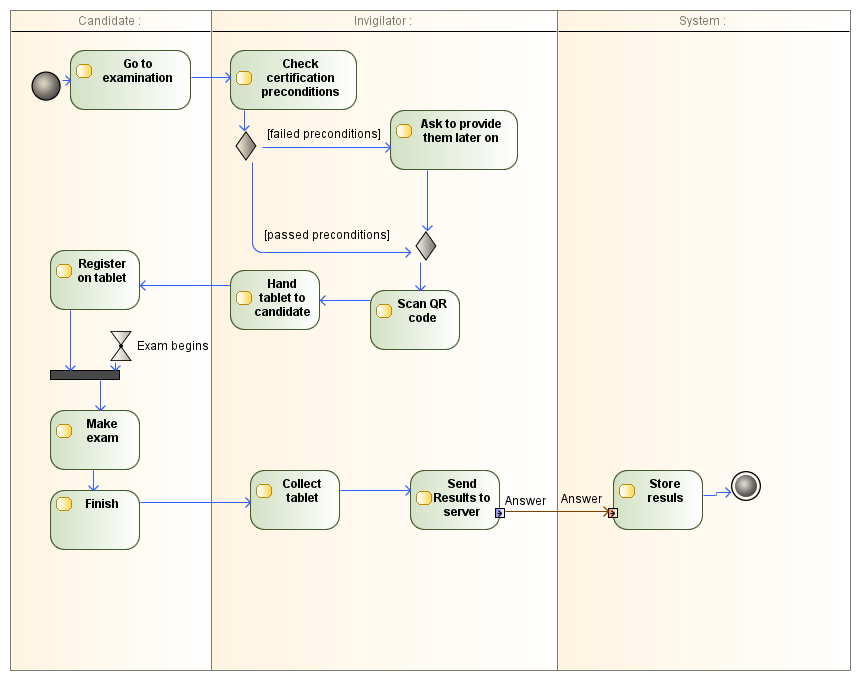
\includegraphics[scale=0.4]{uml/takeexamreq.png}
    \caption{Der Ablauf des Take Exam Usecases im Detail}
    \label{fig:takexdet}
\end{figure}

\subsection{Einbeziehen von Architekturreviewparametern}
Um die Einhaltung der Qualitätsparameter zu garantieren wird empfohlen, dass Architekturreviews durchgeführt werden \cite[S. 20]{review}. Es existiert zwar \glqq keine singuläre, allgemein akzeptierte Metrik um eine Architektur zu beurteilen\grqq \cite[S. 19]{review}, jedoch liefern sie grobe Einschätzungen über die Angemessenheit des Systems \cite[S. 20]{review}. Folgende Architekturreviews wurden dafür ausgewählt:

\begin{itemize}
  \item ATAM: betrachtet Wachstums- und explorative Szenarien um die Architektur zu beurteilen \cite[S. 61]{review}.
  \item CBAM: basiert auf ATAM, beachtet jedoch vor allem den Nutzen, die Risiken und Kosten der Architektur, um die Architekturentscheidungen besser abwägen zu können. Hauptfaktor ist der ROI. \cite[S. 67]{review}
\end{itemize}

Für diese Reviews können bereits früh ein Großteil der benötigten Parameter ermittelt bzw. zumindest grob abgeschätzt werden. Dies ist wichtig, weil nach der Zehner-Regel der Fehlerkosten früh erkannte Fehler und Probleme weniger Kosten nach sich ziehen als später Erkannte \cite[S. 154]{fehler}.

Deswegen wird das Anforderungstemplate um folgende Parameter erweitert:

\begin{itemize}
  \item Earned Value per Month: Wieviel Umsatz der Usecase in einer bestimmten Zeit generiert
  \item Expected Usage: Anzahl der erwarteten NutzerInnen des Systems pro Zeiteinheit
  \item Growth Scenarios: Anzahl der erwarteten NutzerInnen des Systems pro Zeiteinheit bei einer höheren NutzerInnenanzahl und der erwartete Umsatz durch eine Steigerung dieser NutzerInnenzahlen
  \item Change Scenarios: mögliche Änderungsszenarien und Erweiterungen
\end{itemize}

\subsection{Einbeziehen von überprüfbaren, nicht funktionalen Qualitätsattributen}
Nicht funktionale Qualitätsattribute beschreiben die nicht funktionalen Anforderungen an das System. Da diese Qualitäten oft ungenau formuliert sind, ist es wichtig, diese Attribute in einer messbaren Form aufzunehmen \cite[S. 9]{effektiv}.

Deswegen werden für jeden Usecase und dessen architekturrelevanten, nicht funktionalen Anforderungen, messbare Parameter definiert. Diese Parameter sind die Ausgangsbasis für die später folgende Architekturüberprüfung.

Für das Beispielprojekt wurden folgende Parameter definiert, mit welchen das Anforderungstemplate erweitert wurde:

\begin{itemize}
  \item Response Time in Seconds: Wie schnell die Antwort des Systems auf eine Anfrage reagieren muss. Wichtig ist hier die Unterscheidung in zwei Kategorien: ist die Anforderung verbindend oder nur eine Empfehlung.
\end{itemize}

Diese Parameter können von Projekt zu Projekt unterschiedlich sein, je nachdem welche zusätzlichen Einschränkungen vom/von der KundIn ermittelt worden wurden.

\subsection{Ermittlung der Nachbarsysteme und deren Schnittstellen}
Für die Planung der Schnittstellen des Systems sind die Anforderungen und Schnittstellen der Nachbarsysteme von wesentlicher Bedeutung. Die Nachbarsysteme können die Architektur des Systems wesentlich beeinflussen. Ein Beispiel hierfür ist zB. die Frage, ob das Payment System wie in diesem Falle nur eine Schnittstelle zur Abfrage der eingegangenen Zahlungen aufweist, oder ob es ein System nach einer eingangenen Zahlung selbst verständigen kann. Ersteres erfordert eine kontinuierliche Abfrage der Zahlungen, während Zweiteres eine eigens dafür ausgelegt Schnittstelle zur Benachrichtigung der Zahlungen benötigt.

\section{Rahmenbedingungen}
Zusätzlich zu funktionalen und nicht funktionalen Anforderungen werden auch die Rahmenbedingungen ermittelt, unter welchem das System erstellt werden soll. Diese Anforderungen beinhalten meist den organisatorischen und zeitlichen Ablauf des Projektes und können auch gewisse Technologien vorschreiben, zB. wenn das System in ein bereits bestehendes System integriert werden soll. \cite[S. 9]{review}\cite[S. 110]{softarch}

Die Rahmenbedingungen des Beispielprojektes lassen sich zum Großteil aus dem ISO Standard für Personenzertifizierungsstellen ermitteln \cite{ISO_CERT} und geben Einsicht in die Vertraulichkeit der Daten. Daraus eröffnen sich weitere Usecases. Sofern möglich werden diese Parameter in das Usecasediagramm und das Klassendiagramm der zu verwendeten Daten mit einbezogen. Auf zeitliche und technologische Rahmenbedingungen wurde im Beispielprojekt nicht eingegangen.

\section{Ermittlung der Daten}
Die verwendeten Daten werden ermittelt und mit Hilfe eines Klassendiagramms modelliert. Dies ist nicht nur wichtig und nützlich, um einen Überblick über die Parameter der zu erstellenden Interfaces zu erhalten, sondern wird später auch einen wesentlichen Beitrag zur Aufteilung des Systems in Komponenten leisten. Im Falle des Beispielprojekts wurden folgende Daten ermittelt und modelliert:

\begin{figure}[H]
    \centering
    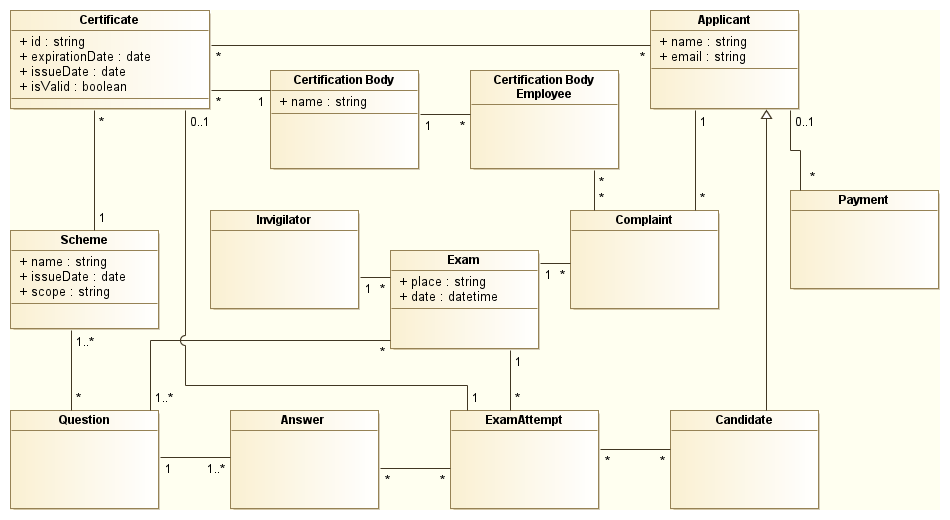
\includegraphics[scale=0.5]{uml/class.png}
    \caption{Das ermittelte Klassendiagramm des Beispielprojektes}
\end{figure}

\section{Ermittlung der Netzwerke}
Nach der Ermittlung der Daten wird auf Basis der Rahmenbedingungen und Sicherheitsstruktur zusammen mit dem/der Kunden/Kundin ermittelt, welche Netzwerke für das System benötigt werden. Netzwerke stellen eigene abgeschlossene Bereiche dar, in welchen das System operiert oder von welchem auf das System zugegriffen werden kann. Grundsätzlich existiert mindestens ein Netzwerk. In diesem Fall beherbergt diese Netzwerke das interne System des Unternehmens.

Soll von anderen Systemen, zB. vom Internet auf Funktionalitäten des Systems zugegriffen werden können, wird ein weiteres Netzwerk benötigt.

Aus den Usecases des Beispielprojektes lässt sich ermitteln, dass in diesem Falle mindestens zwei Netzwerke benötigt werden:

\begin{itemize}
  \item Public: Usecases die vom Internet auf das System zugreifen, zB. wenn sich ein/eine AnwärterIn (Applicant) für eine Prüfung registriert
  \item Internal: Usecases, welche nicht vom Internet aus zugänglich sind
\end{itemize}

Die Netzwerke werden nun mit einer Vertrautheitsebene von 1 bis n versehen, um eine Sicherheitshirarchie der Netzwerke zu generieren. Es kann vorkommen, dass mehrere Netzwerke mit der selben Vertrautheitsebene versehen werden, diese dürfen sich jedoch nicht überlappen. Zum Beispiel könnte eine weitere Niederlassung der Firma ein eigenes System erstellen, auf welches man auch vom Internet aus zugreifen kann. Das Internet würde dann mit der Vertrautheitsebene 1 versehen und beide Systeme mit der Ebene 2. Überlappen sich diese Systeme, muss das überlappende Netzwerk in ein eigenes System ausgegliedert werden.

Die ermittelten Daten werden nun Netzwerken zugeteilt, für welche sie essentiell zum Betrieb des Systems sind. Auch die AkteurInnen werden in Netzwerke aufgeteilt, in welchen sie operieren. Scheinen Daten oder AkteurInnen in mehreren Netzwerke auf, werden sie dem Netzwerk mit der höchsten Sicherheitsebene zugeteilt. Die niedrigeren Bereiche können dann auf diese Bereiche anhand von festgelegten APIs zugreifen.

Im Falle des Beispielprojektes werden alle aufgenommen Daten im Internal Netzwerk verwaltet, da alle Daten als businesskritisch für das Internal System angesehen werden, welches wiederum die höchste Sicherheitsebene besitzt. Würde das Beispielprojekt zB. um ein Forum oder einen Blog erweitert, würden diese dem Public Netzwerk zugeteilt werden; AkteurInnen des Internal Systems können zwar auch auf diese Forum zugreifen oder Blogeinträge schreiben, jedoch sind diese Aktivitäten und Daten nicht kritisch für den normalen Betrieb des Internal Systems. Würde das Forum oder der Blog gehackt werden, resultiert dies zwar in einem Schaden für das Unternehmen, das Internal System könnte aber auch weiterhin normal operiert werden.

Nach der generellen Aufteilung der Daten wird eine Analyse der Rahmenbedingungen durch geführt, um zu erfahren, ob bestimmte Daten aufgrund von Richtlinien besonders geschützt, und somit in eine eigenes Netzwerk mit einer höheren Vertrautheitsebene ausgelagert werden müssen. Das Beispielprojekt verlangt die vertrauliche Verarbeitung von Prüfungsergebnissen und erwähnt auch explizit das Personal der Prüfungsstelle \cite[7.3]{ISO_CERT}. Weil das Internal Netzwerk, in welchem das Personal operiert, das Netzwer mit der höchsten Vertrautheitsebene darstellt, muss ein weiteres Netzwerk mit einer höheren Vertrautheitsebene erstellt werden. Dieses Netzwerk wird in diesem Falle mit der Vertrautheitsebene 3 versehen und unter der Beschreibung Confidential geführt.

Um diese Netzwerke besser zu visualisieren zu können, wird das UML Metamodell mit Hilfe eines Profiles angepasst. Jede Netzwerk erhält einen gleich lautenden Stereotypen \cite[S. 518]{glasklar}:

\begin{figure}[H]
    \centering
    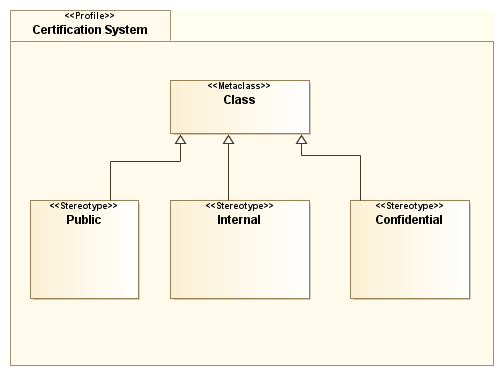
\includegraphics[scale=0.5]{uml/datastereotypes.png}
    \caption{Das Metamodell wird mit einem Profil um drei Stereotypen erweitert, welche die Netzwerke der Applikation darstellen}
\end{figure}

Zusätzlich werden diese Netzwerke auch mit Vertrautheitsebenen verbunden. Diese Ebenen werden im Profil mit einer Notiz versehen, welche die Ebene angibt.

\begin{figure}[H]
    \centering
    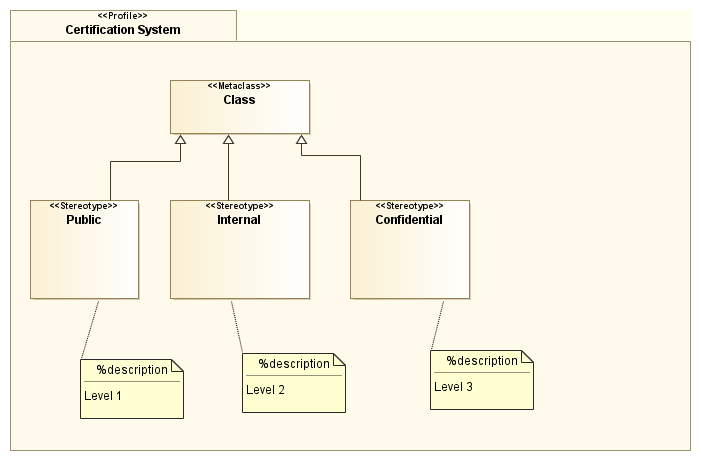
\includegraphics[scale=0.5]{uml/datastereotypeslevel.png}
    \caption{Die Netzwerke werden mit Vertrautheitsebenen versehen}
\end{figure}

Sind die Stereotypen erstellt und mit Vertrautheitsebenen versehen, kann nun damit begonnen werden, die AkteurInnen des Usecasediagramms und die Daten des Klassendiagramms mit diesen Stereotypen zu versehen.

\begin{figure}[H]
    \centering
    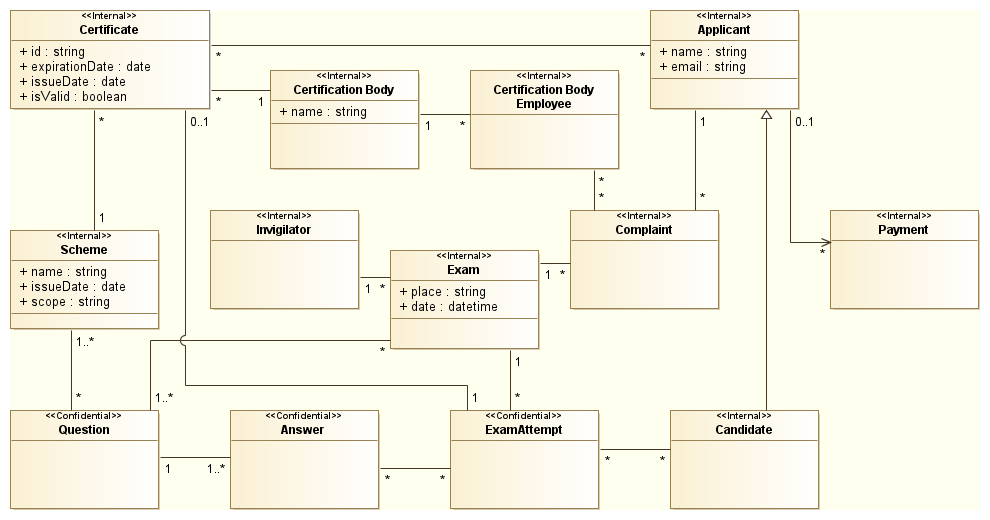
\includegraphics[scale=0.5]{uml/classstereotyped.png}
    \caption{Das Klassendiagramm wird mit Stereotypen der Vertraulichkeit erweitert}
\end{figure}

\begin{figure}[H]
    \centering
    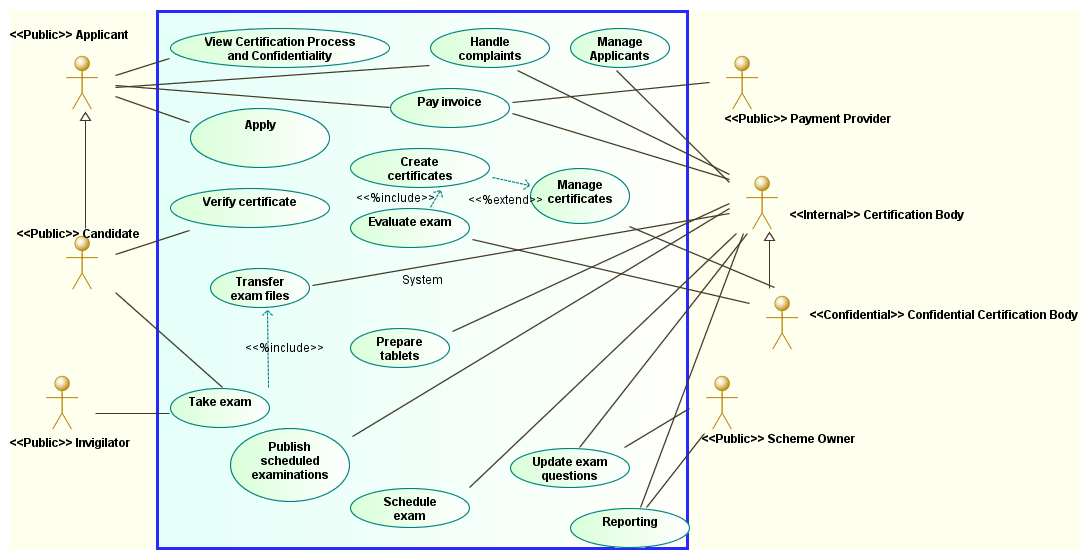
\includegraphics[scale=0.4]{uml/stereotypedusecase.png}
    \caption{Die AkteurInnen des Usecasediagramms wird mit Stereotypen der Vertraulichkeit erweitert}
\end{figure}

\section{Ermittlung der Beziehungen zwischen AkteurInnen, Partnersystemen und Daten}
Auf Basis des Usecasediagramms können die AkteurInnen und deren Partnersysteme mit Hilfe eines Kontextdiagramms visualisiert werden. Im Gegensatz zum Usecasediagramm geht das Kontextdiagramm auf die zwischen den Systemen und AkteurInnen fließenden Daten ein und stellt so die Verbindungen zwischen Daten, Systemen und NutzerInnen auf.

\begin{figure}[H]
    \centering
    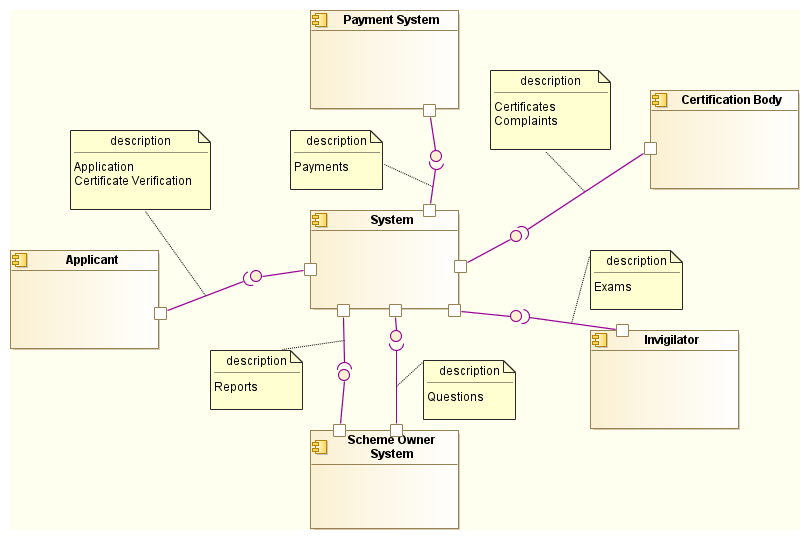
\includegraphics[scale=0.5]{uml/context.png}
    \caption{Das Kontextdiagramm zeigt das System, die AkteurInnen, die Nachbarsysteme und die dazwischen fließenden Daten}
\end{figure}